\def \Qa % 1
{
\begin{textarea}[]
	\only<1>{
		\centering
		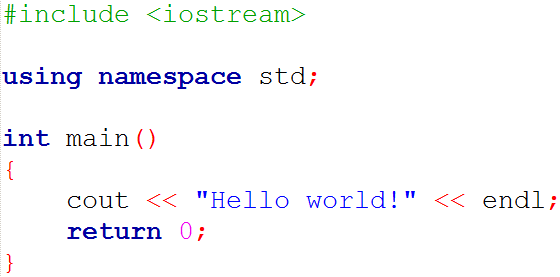
\includegraphics[width=0.8\textwidth]{../categories/media/helloworld/Hello_World_C++.png}
	}
	\only<2>{
		What is ``Hello World'' in C++?
	}
\end{textarea}
}


\def \Qb % 2
{
\begin{textarea}[]
	\only<1>{
		\centering
		%\includegraphics[height=0.5\linewidth]{categories/media//helloworld/whitespace.png}
		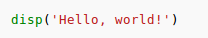
\includegraphics[height=0.11\linewidth]{../categories/media/helloworld/matlab.png}
	}
	\only<2>{
		What is ``Hello World'' in Matlab?
	}
\end{textarea}
}

\def \Qc % 3
{
\begin{textarea}[]
	\only<1>{
		\centering
		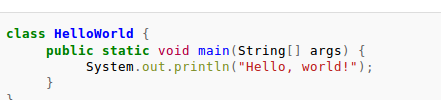
\includegraphics[width=0.7\textwidth]{../categories/media/helloworld/java.png}
	}
	\only<2>{
		What is ``Hello World'' in Java?
	}
\end{textarea}
}

\def \Qd % 4
{
\begin{textarea}[]
	\only<1>{
		\centering
		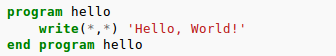
\includegraphics[scale = 0.8]{../categories/media/helloworld/fortran90.png}
	}
	\only<2>{
		What is ``Hello World'' in Fortran 90/95?
	}
\end{textarea}
}

\def \Qe % 5 DOUBLE
{
\begin{textarea}[]
	\only<1>{
		\centering
		\includegraphics[height=0.5\linewidth]{../categories/media/helloworld/whitespace.png}
	}
	\only<2>{
		What is ``Hello World'' in Whitespace?
	}
\end{textarea}
}
